%--------------------------------------------------
\section{Aplicación Interactiva para el Personal de Ventas (AIPV)}


La Aplicación Interactiva para el Personal de Ventas tiene como objetivo ser un apoyo al vendedor para conocer más sobre las preferencias de un cliente, poder otorgarle una atención personalizada y/o asistirlo en la elección de la compra de un producto. \\ \par
La figura \ref{arq-AIPV}  presenta la arquitectura de este módulo.
\FloatBarrier
\begin{figure}[htbp!]
		\centering
			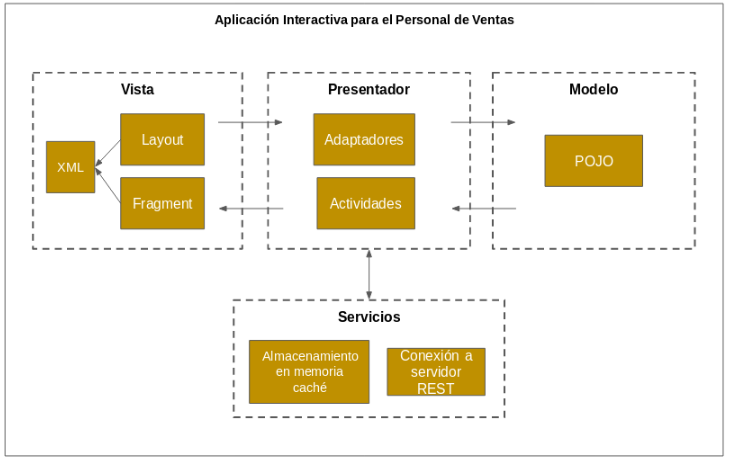
\includegraphics[width=.9 \textwidth]{imagenes/Arquitecturas/arquiVendedor}
		\caption{Arquitectura del módulo AIPV.}
		\label{arq-AIPV}
\end{figure}
\FloatBarrier

%--------------------------------------------------
\subsection{Prototipo 1: Diseño inicial de la aplicación y descubrimiento de Beacons}

%introducción%
El prototipo 1 de la aplicación incluye el diseño inicial de la misma, así como el descubrimiento de los Beacons dentro del comercio, con el fin de mantener un registro de donde se encuentran. Para ello Estimote nos permite crear zonas de proximidad mediante claves - valor que se establecen en el Beacon, cuando el usuario vendedor entra en una de estas zonas de proximidad la aplicación envía la ubicación para registrar las coordenadas actuales del Beacon.  \\ \par

%--------------------------------------------------
\subsubsection{Análisis}

Dentro del análisis para el desarrollo de este prototipo se incorporan los requerimientos funcionales \hyperlink{RFAPV}{RFAPV1 Iniciar sesión} y \hyperlink{RFAPV}{RFAPV2 Enviar de ubicación de Beacons}, definidos previamente en el capítulo del ``Bosquejo general de la aplicación''  con el título de ``Requerimientos funcionales de la Aplicación Interactiva para el Personal de Ventas''. \\ \par

\paragraph{Casos de uso de la AIPV.} ~\\

La figura \ref{casos-uso-AIPV1} muestra los casos de uso del prototipo 1 de la AIPV.

\FloatBarrier
\begin{figure}[htbp!]
		\centering
			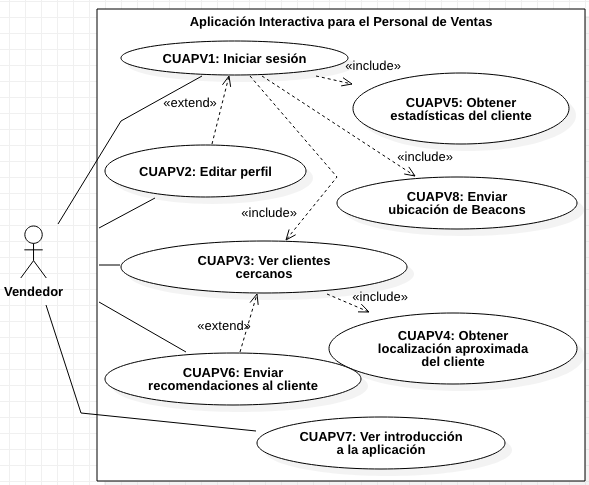
\includegraphics[width=.9 \textwidth]{imagenes/adrian/vendedor/prototipo1/casos_de_uso}
		\caption{Casos de uso de la AIPV.}
		\label{casos-uso-AIPV1}
\end{figure}
\FloatBarrier

\paragraph{Diagrama de clases.} ~\\

La figura \ref{clases-AIPV1} presenta el diagrama de clases para el prototipo 1 de la AIPV. Para una mejor visualización, el diagrama se ha dividido en 3 partes. 

\FloatBarrier
\begin{figure}[htbp!]
		\centering
			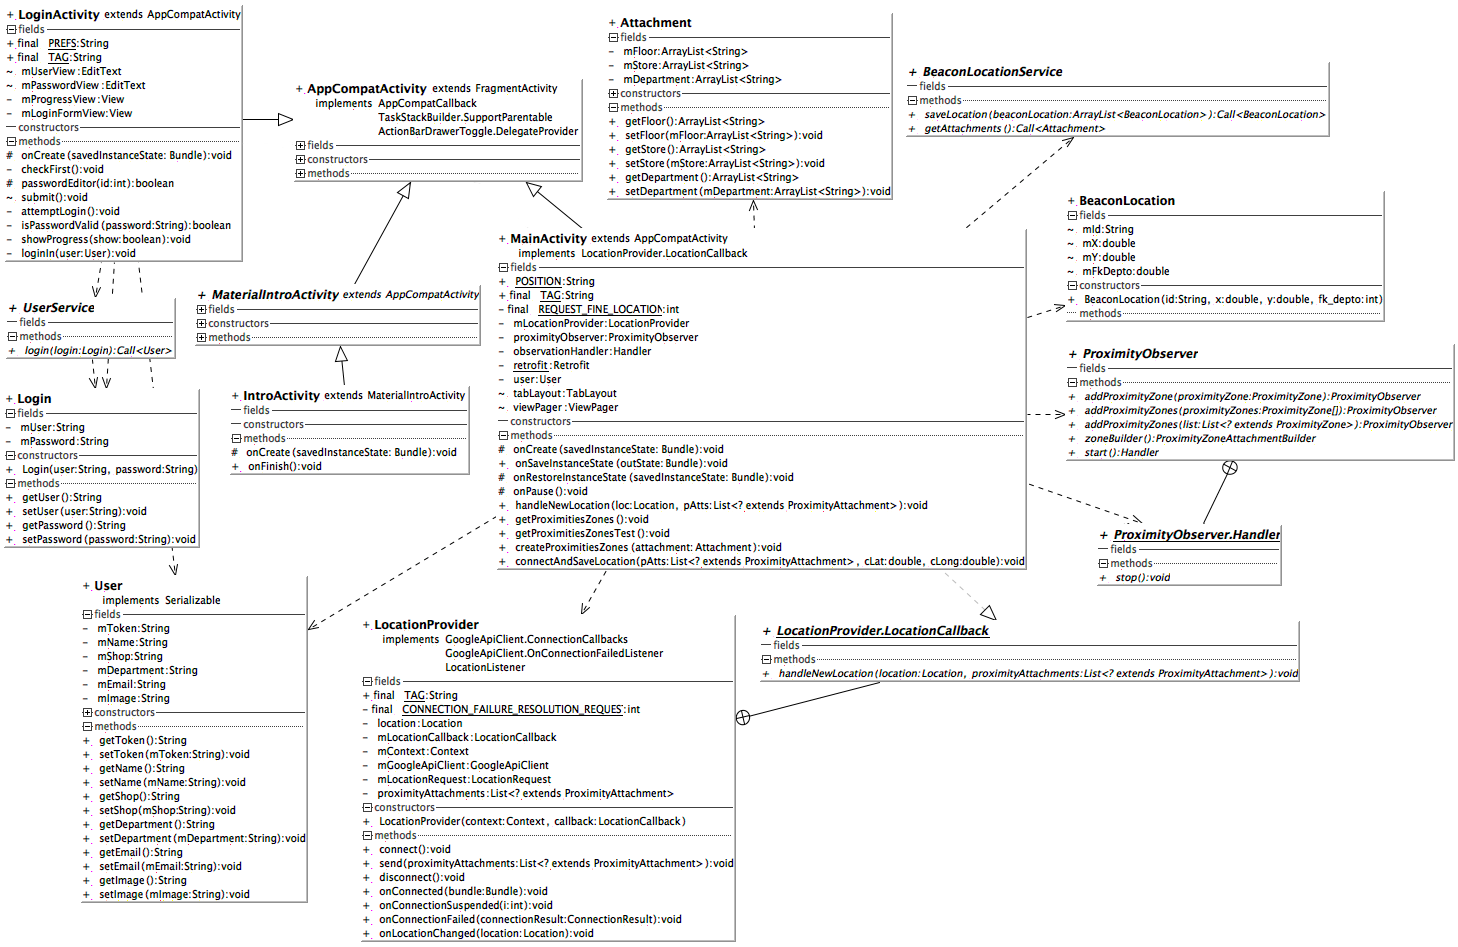
\includegraphics[width=.9 \textwidth]{imagenes/adrian/vendedor/prototipo1/clases}
		\caption{Diagrama de clases del prototipo 1 de la AIPV (Visualización completa).}
		\label{clases-AIPV1}
\end{figure}
\FloatBarrier

La descripción de los elementos de la parte 1 del diagrama de clases es la siguiente: 


\begin{itemize}
\item \textbf{AppCompatActivity}: Clase base para actividades que utilizan las características de la barra de acciones de la biblioteca de soporte de Android.
\item \textbf{LoginActivity}: Clase encargada del inicio de sesión, solicita el nombre de usuario y contraseña al vendedor, utiliza la interfaz UserService para hacer una petición POST al servidor y comprobar que los datos sean correctos para un inició de sesión exitoso.
\item \textbf{UserService}: Interfaz que define el método login, esta interfaz utiliza retrofit que nos permite consumir la API REST en la aplicación.
\item \textbf{Login}: Clase que retrofit convierte y coloca en el cuerpo de una petición HTTP POST, contiene el nombre de usuario y contraseña proporcionados por el vendedor.
\item \textbf{IntroActivity}: Clase encargada de mostrar una pequeña introducción de lo que es posible realizar el vendedor desde la aplicación. Extiende de la clase MaterialIntroActivity.
\item \textbf{MainActivity}: Clase principal de la aplicación, en ella se muestra la lista de usuarios cercanos y el fragmento para editar el perfil del vendedor. Implementa la interfaz LocationProvider.LocationCallback para obtener la localización de un Beacon al entrar a una zona de proximidad, además de usar la interfaz BeaconLocationService para hacer una petición GET y obtener las claves - valor necesarias para generar las zonas de proximidad, también se utiliza la misma interfaz para hacer una petición POST al servidor y guardar la ubicación.
\item \textbf{Attachment}: Clase que retrofit mapea, es la respuesta de una petición HTTP GET en formato JSON, contiene arreglos de String para generar zonas de proximidad por pisos, tiendas o departamentos.
\end{itemize}

La figura \ref{clases-AIPV1-parte1} contiene las clases previamente descritas.


\FloatBarrier
\begin{figure}[htbp!]
		\centering
			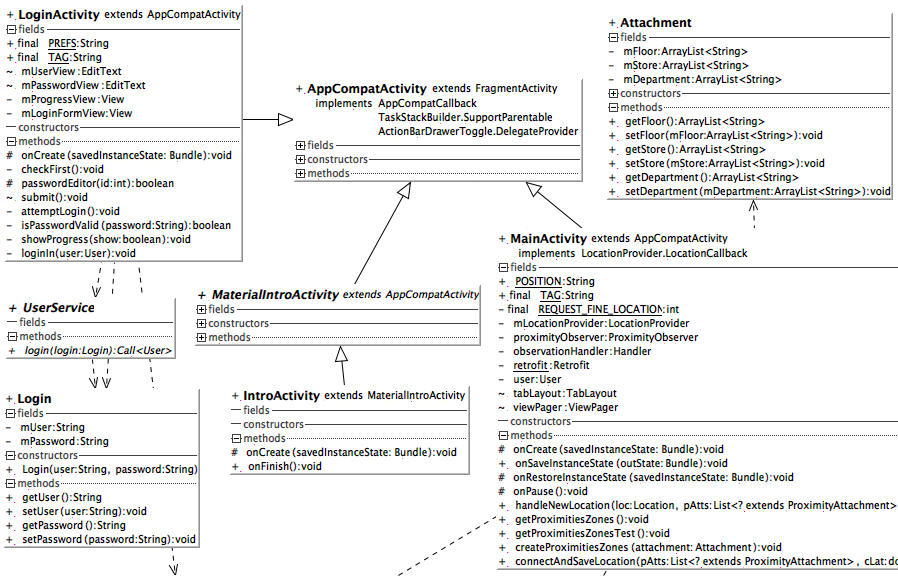
\includegraphics[width=1 \textwidth]{imagenes/adrian/vendedor/prototipo1/clases_1}
		\caption{Diagrama de clases del prototipo 1 de la AIPV (Parte 1) .}
		\label{clases-AIPV1-parte1}
\end{figure}
\FloatBarrier

La descripción de los elementos de la parte 2 del diagrama de clases es la siguiente: 

\begin{itemize}
\item \textbf{BeaconLocationService}: Interfaz que define el método saveLocation para guardar la ubicación actual de Beacons y el método getAttachments que obtiene las claves - valor necesarias para generar las zonas de proximidad, esta interfaz utiliza retrofit que nos permite consumir la API REST en la aplicación.
\item \textbf{BeaconLocation}: Clase en la que se guarda el id de un Beacon y su ubicación actual, se envía en un ArrayList el cual retrofit convierte y coloca en el cuerpo de una petición HTTP POST.
\item \textbf{ProximityObserver}: Interfaz de Estimote que define los métodos para agregar zonas de proximidad en la aplicación y comenzar el descubrimiento de Beacons.
\item \textbf{LocationProvider.LocationCallback}: Interfaz que define el método handleNewLocation que se encarga de vincular una lista de Beacons con una localización.

\end{itemize}

La figura \ref{clases-AIPV1-parte2} contiene las clases previamente descritas.

\FloatBarrier
\begin{figure}[htbp!]
		\centering
			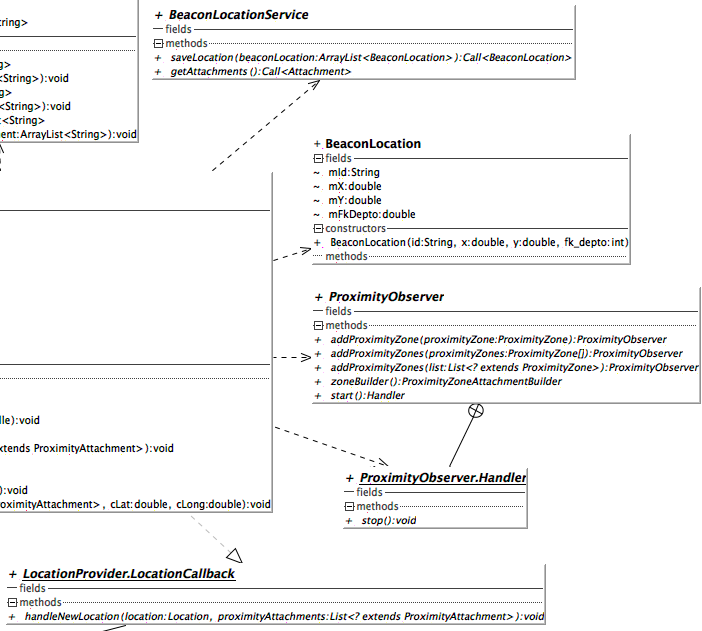
\includegraphics[width=.9 \textwidth]{imagenes/adrian/vendedor/prototipo1/clases_2}
		\caption{Diagrama de clases del prototipo 1 de la AIPV (Parte 2).}
	     \label{clases-AIPV1-parte2}
\end{figure}
\FloatBarrier

La descripción de los elementos de la parte 3 del diagrama de clases es la siguiente: 

\begin{itemize}
\item \textbf{User}: Clase que retrofit mapea, es la respuesta de la petición HTTP POST para el inicio de sesión la cual está en formato JSON, contiene la información básica del usuario vendedor.
\item \textbf{LocationProvider}: Clase que obtiene la geolocalización del dispositivo móvil mediante la clase LocationRequest de Google Play Services.

La figura \ref{clases-AIPV1-parte3} contiene las clases previamente descritas.

\end{itemize}
\FloatBarrier
\begin{figure}[htbp!]
		\centering
			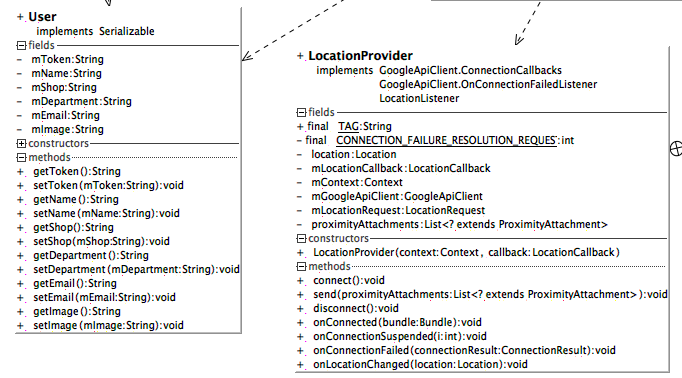
\includegraphics[width=.9 \textwidth]{imagenes/adrian/vendedor/prototipo1/clases_3}
		\caption{Diagrama de clases del prototipo 1 de la AIPV (Parte 3).}
		\label{clases-AIPV1-parte3}
\end{figure}
\FloatBarrier

%--------------------------------------------------
\subsubsection{Diseño}

%introducción%
A partir de los requerimientos definidos para este prototipo se muestran los casos de uso, diagramas de secuencia, el flujo de navegación y las interfaces de la aplicación.\\ \par

\title{\textbf{Diagramas de secuencia}\\}

\title{\textbf{Iniciar sesión.}\\}

En la figura \ref{secuencia-AIPV1-inicio} se muestra el diagrama de secuencia para iniciar sesión en la AIPV, el cual describe los pasos que se llevan  a cabo para que el usuario vendedor inicie sesión satisfactoriamente.

\FloatBarrier
\begin{figure}[htbp!]
		\centering
			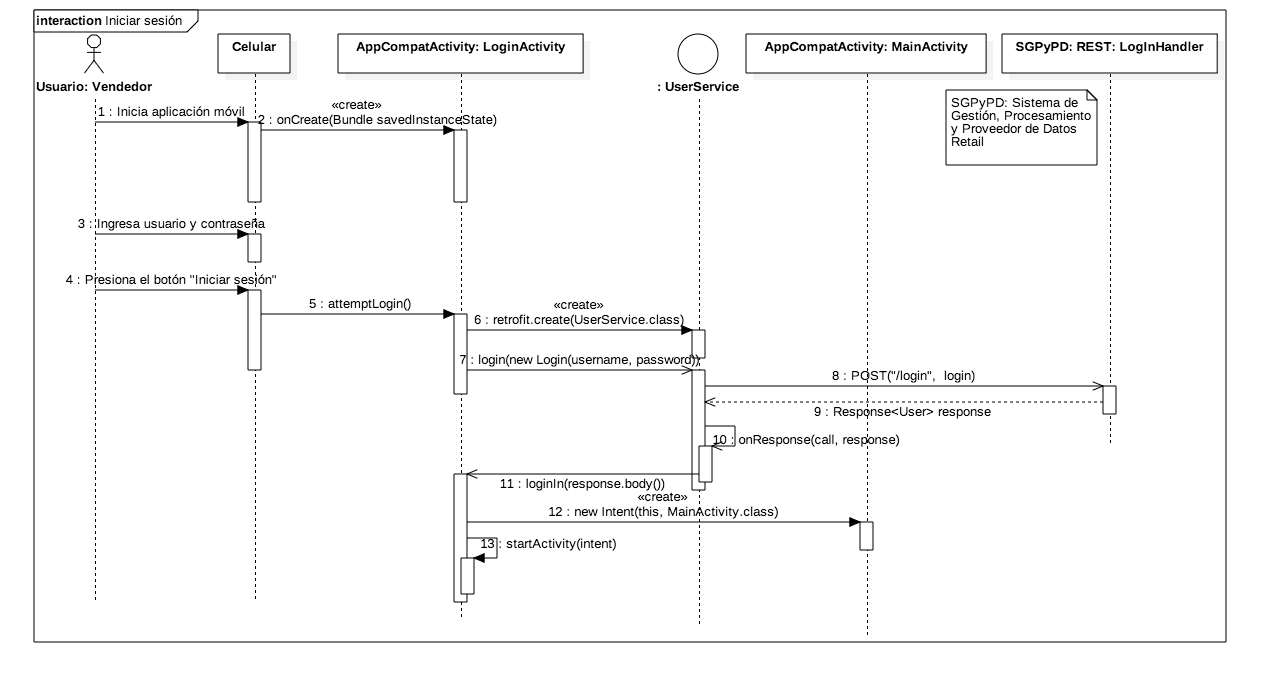
\includegraphics[width=1.1 \textwidth]{imagenes/adrian/vendedor/prototipo1/inicio_de_sesion}
		\caption{Diagrama de secuencia para el inicio de sesión de un vendedor.}
		\label{secuencia-AIPV1-inicio}
\end{figure}
\FloatBarrier


\title{\textbf{Ver introducción a la aplicación.}\\}

En la figura \ref{secuencia-AIPV1-intro} se muestra el diagrama de secuencia para ver una introducción a la AIPV, es decir, mostrarle al usuario vendedor lo que es posible realizar dentro de la aplicación.
 
\FloatBarrier
\begin{figure}[htbp!]
		\centering
			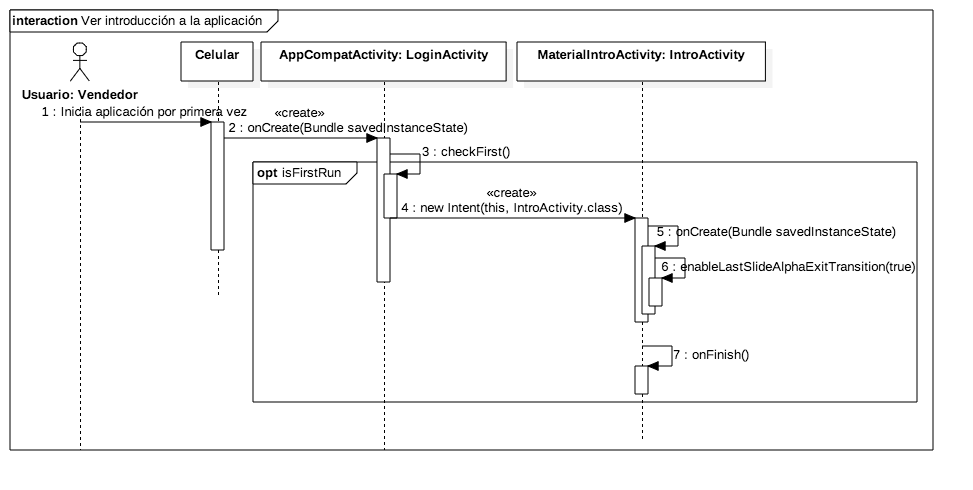
\includegraphics[width=1.1 \textwidth]{imagenes/adrian/vendedor/prototipo1/intro_app}
		\caption{Diagrama de secuencia para ver una introducción a la aplicación.}
		\label{secuencia-AIPV1-intro}
\end{figure}
\FloatBarrier

\title{\textbf{Enviar ubicación de Beacons.}\\}

En la figura \ref{secuencia-AIPV1-Beacons} se muestra el diagrama de secuencia para enviar la ubicación de los Beacons desde la AIPV, el cual describe los pasos que se llevan a cabo para que la aplicación cree las zonas de proximidad y pueda detectar correctamente los Beacons, para una mejor visualización el diagrama se ha dividido en 2 partes las cuales se muestran en las figuras \ref{secuencia-AIPV1-BeaconsUno} y \ref{secuencia-AIPV1-BeaconsDos}.

\FloatBarrier
\begin{figure}[htbp!]
		\centering
			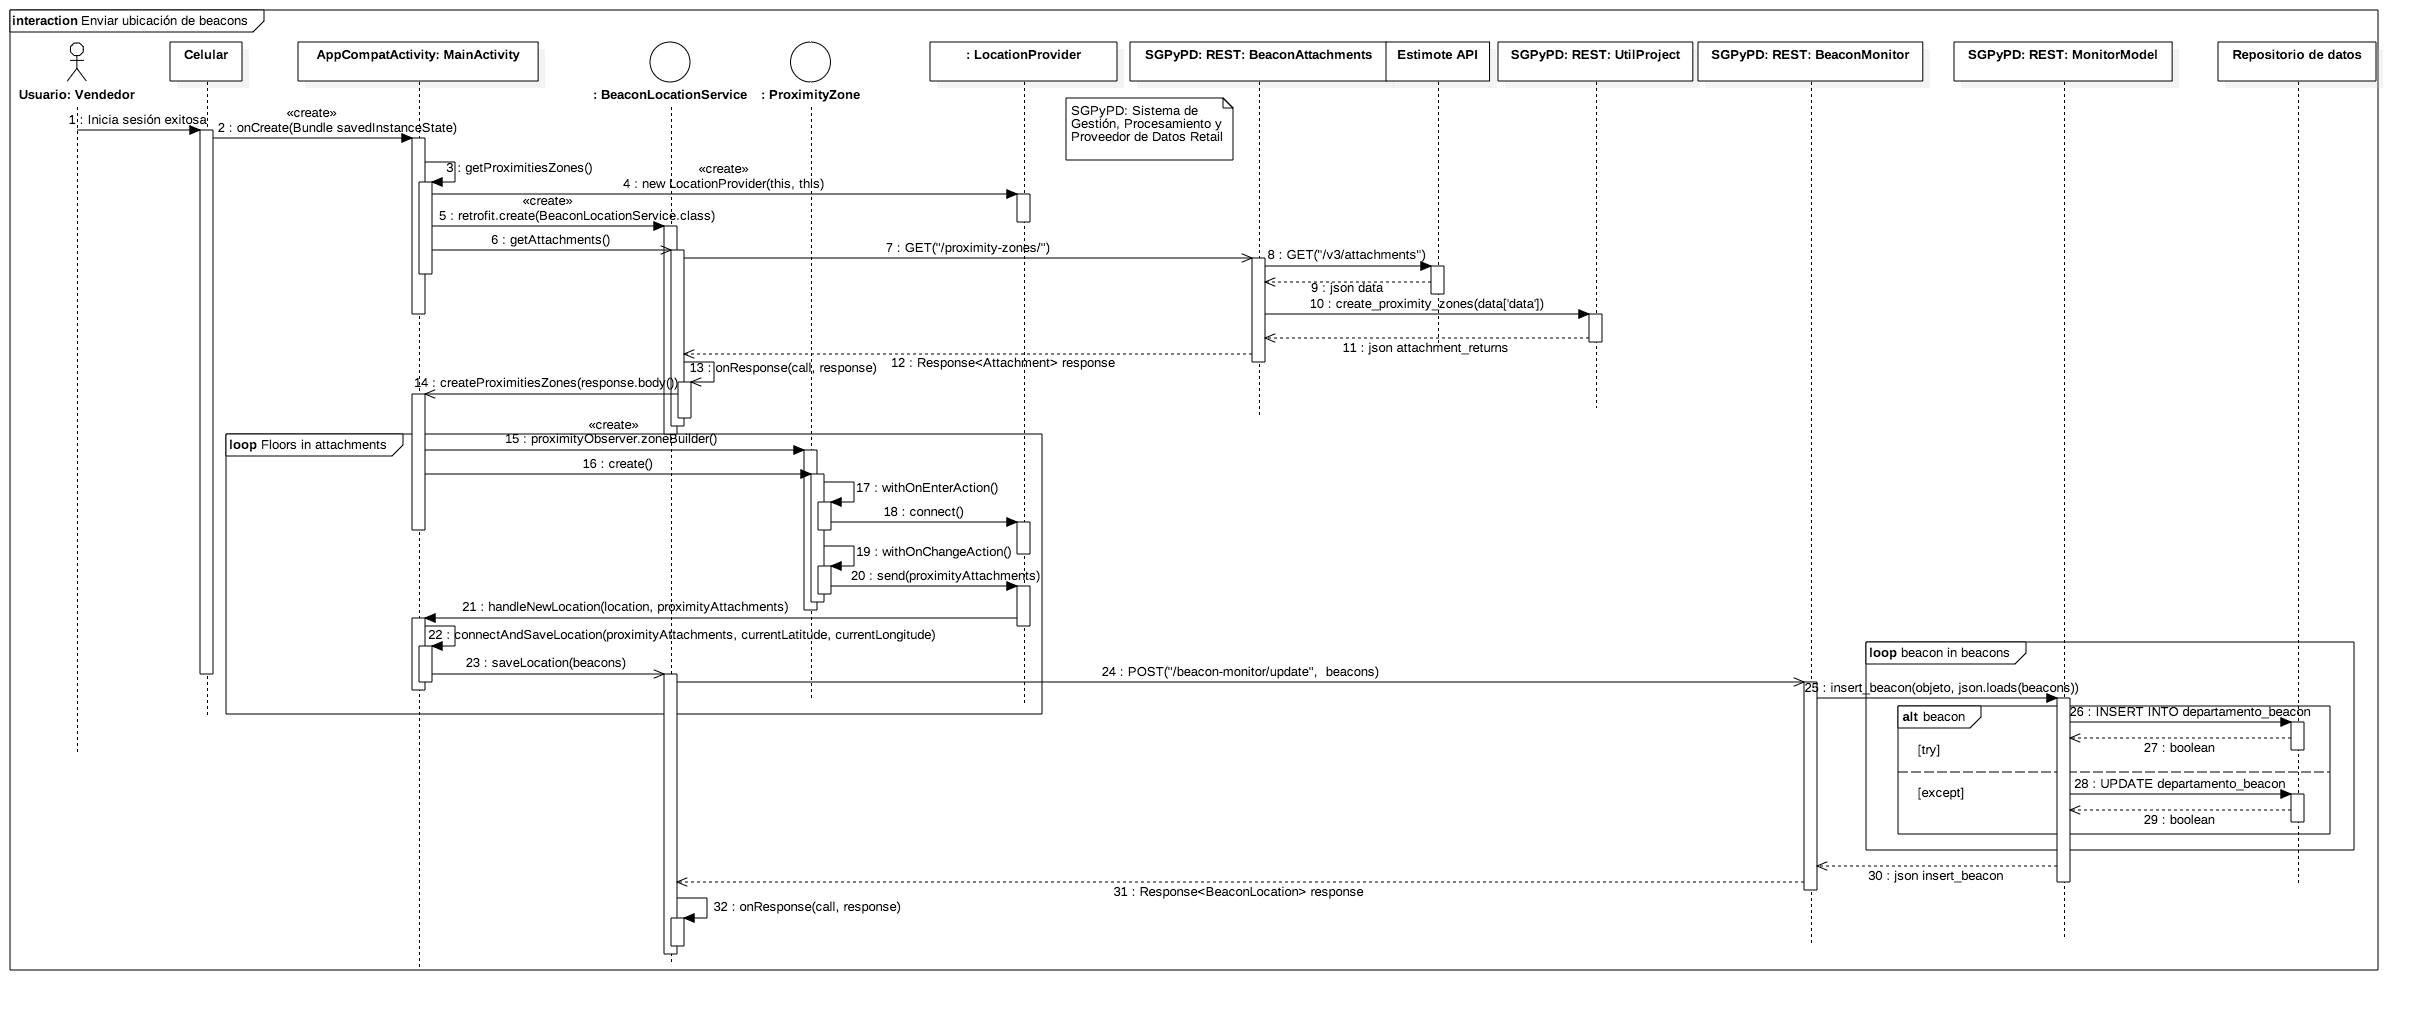
\includegraphics[width=1 \textwidth]{imagenes/adrian/vendedor/prototipo1/enviar_Beacons}
		\caption{Diagrama de secuencia para enviar la ubicación de Beacons (Visualización completa).}
		\label{secuencia-AIPV1-Beacons}
\end{figure}
\FloatBarrier

\FloatBarrier
\begin{figure}[htbp!]
		\centering
			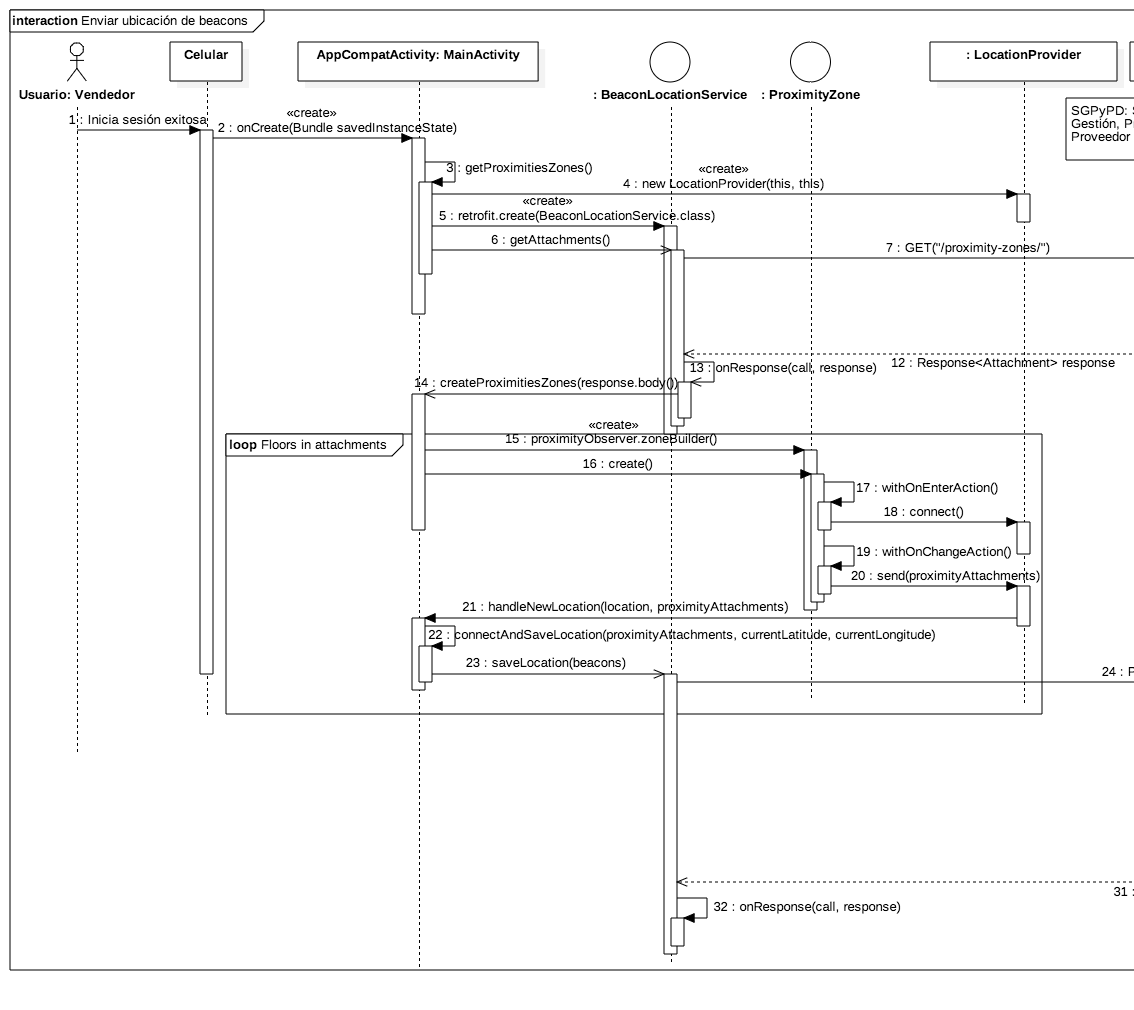
\includegraphics[width=1 \textwidth]{imagenes/adrian/vendedor/prototipo1/enviar_Beacons_1}
		\caption{Diagrama de secuencia para enviar la ubicación de Beacons (Parte 1).}
		\label{secuencia-AIPV1-BeaconsUno}
\end{figure}
\FloatBarrier

\FloatBarrier
\begin{figure}[htbp!]
		\centering
			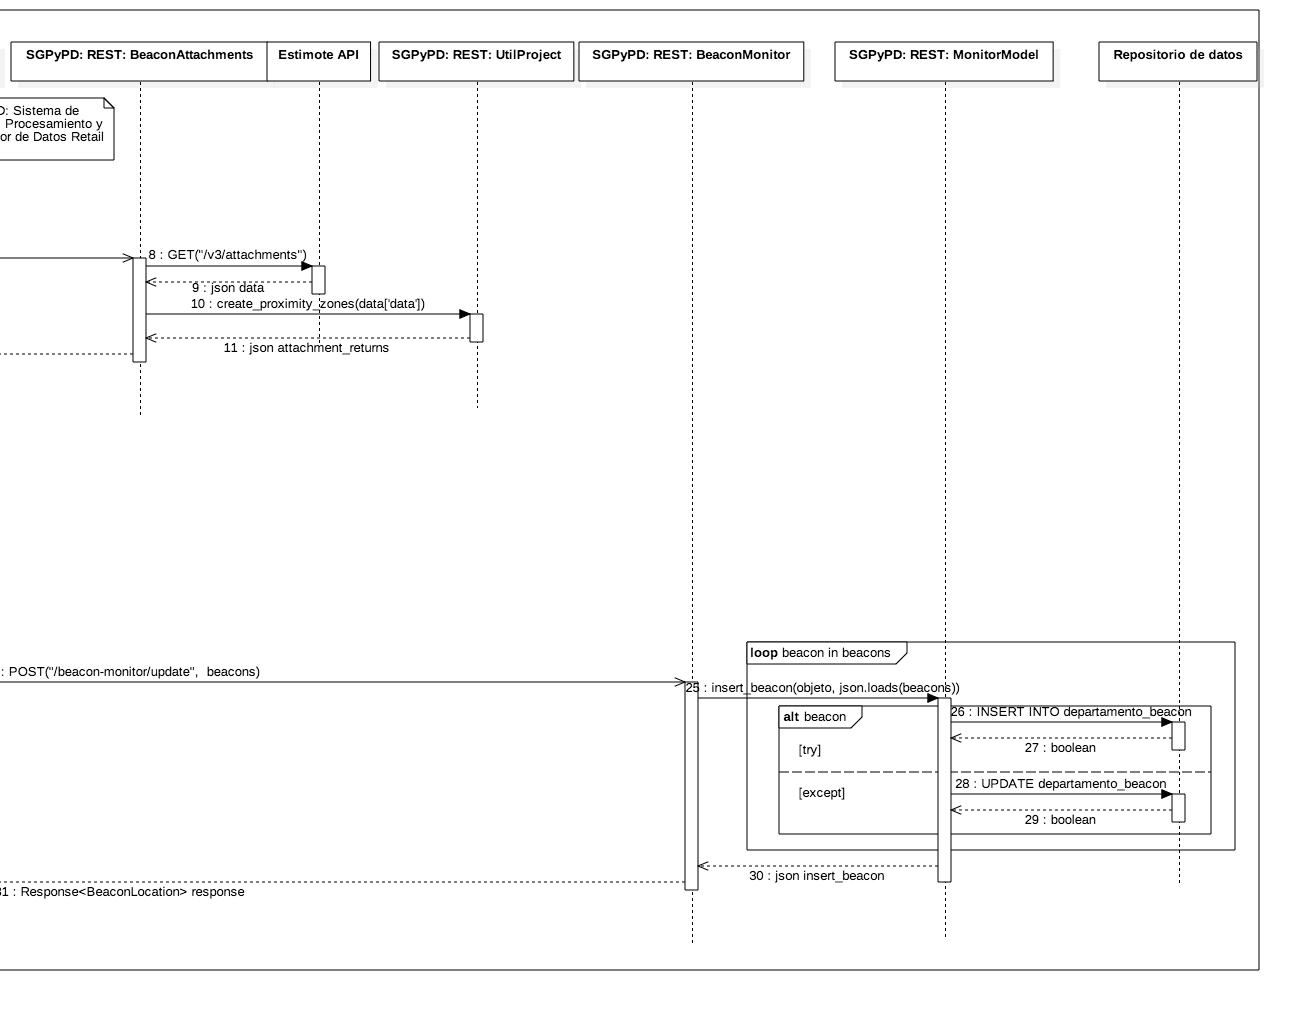
\includegraphics[width=1 \textwidth]{imagenes/adrian/vendedor/prototipo1/enviar_Beacons_2}
		\caption{Diagrama de secuencia para enviar la ubicación de Beacons (Parte 2).}
		\label{secuencia-AIPV1-BeaconsDos}
\end{figure}
\FloatBarrier
\paragraph{Flujo de navegación de la AIPV.} ~\\

La siguiente figura \ref{navegacion-AIPV1} muestra como es el flujo de navegación de la aplicación.

\FloatBarrier
\begin{figure}[htbp!]
		\centering
			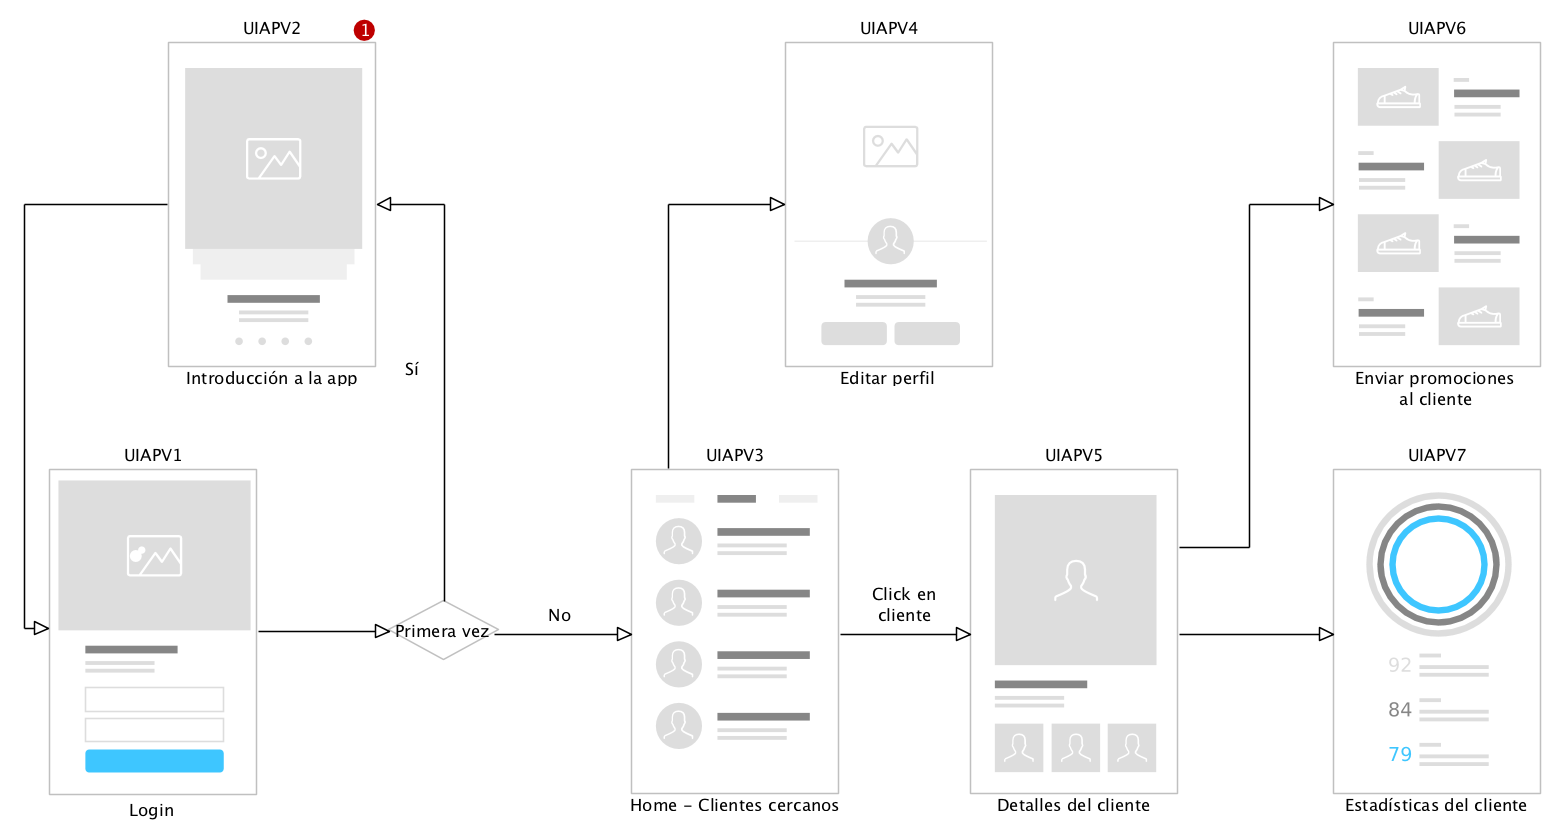
\includegraphics[width=1 \textwidth]{imagenes/adrian/vendedor/prototipo1/UIApp/0}
		\caption{Flujo de navegación de la AIPV.}
		\label{navegacion-AIPV1}
\end{figure}

\paragraph{Interfaces de usuario}

\cfinput{appMovil/Vendedor/prototipo1/UI/UIAPV1}
\cfinput{appMovil/Vendedor/prototipo1/UI/UIAPV2}
\cfinput{appMovil/Vendedor/prototipo1/UI/UIAPV3}
\cfinput{appMovil/Vendedor/prototipo1/UI/UIAPV4}
\cfinput{appMovil/Vendedor/prototipo1/UI/UIAPV5}
\cfinput{appMovil/Vendedor/prototipo1/UI/UIAPV6}
\cfinput{appMovil/Vendedor/prototipo1/UI/UIAPV7}

%casos de uso%

%interacción de la navegación%

